%\documentclass[authoryear,round]{tufte-book}
\documentclass[a4paper,10pt]{article}
\usepackage[T1]{fontenc}
\usepackage[utf8]{inputenc}
\usepackage{amsmath}
\usepackage{amssymb}
\usepackage{graphicx}
\usepackage{fullpage}
\usepackage{color}
\usepackage{natbib}
\usepackage{mathrsfs}
\usepackage{array}
\newcommand{\head}[2]{\multicolumn{1}{>{\centering\arraybackslash}p{#1}}{#2}}
%\usepackage{sidecap}
\usepackage[capbesideposition={top,right},facing=yes,capbesidesep=quad]{floatrow}
\usepackage[hypertexnames=false]{hyperref}
\hypersetup{colorlinks=true, urlcolor=blue, citecolor=black, linkcolor=black}
%\usepackage{lineno}
%\usepackage{lscape}
%\usepackage{multirow}

\newcommand{\var}{\mathop{\mbox{Var}}}
\newcommand{\cov}{\mathop{\mbox{Cov}}}
\newcommand{\fancyN}{$\mathcal N$ }
\newcommand{\fancyB}{$\mathcal B$ }
\newcommand{\gc}[1]{{\it \color{red} (#1)} }
\newcommand{\jb}[1]{{\it\color{blue} (#1)} }
\def\citeapos#1{\citeauthor{#1}'s (\citeyear{#1})}
%\newcommand{\Rho}{\mathrm{P}}

%opening
\title{Theory of Sweeps from Standing Variation}
\author{
Jeremy J. Berg$^{1,2,3}$ and Graham Coop$^{1,2,3}$ \\
$^1$ Graduate Group in Population Biology, University of California, Davis. \\
$^2$ Center for Population Biology, University of California, Davis.\\
$^3$ Department of Evolution and Ecology, University of California, Davis\\
\small To whom correspondence should be addressed: \texttt{jjberg@ucdavis.edu, gmcoop@ucdavis.edu}\\
}

\date{}

\begin{document}

%\linenumbers
\maketitle

\begin{abstract}
\end{abstract}

%%%%%%%%%%%%%%%%%%%%%%%%%%%
\section{Introduction}

During the last few decades, an understanding of how positive directional selection and the associated genetic hitchhiking effect influence patterns of genetic variation has become a valuable tool for evolutionary geneticists. The characteristic reductions in genetic diversity and long extended haplotypes that are left behind in the wake of a selective sweep allow for both the identification of individual genes that have contributed to recent adaptation within a population (i.e. hitchhiking mapping), and for understanding the rate and dynamics of adaptation at a genome-wide level \jb{REFS}.

While the contribution of many different modes to the adaptive process has long been recognized \jb{REFS},  early work on the hitchhiking effect focused largely on the scenario where a single co-dominant mutation arose and was immediately beneficial, rapidly sweeping to fixation. However, there are many empirical examples which violate this simple model, where selection acts on standing variation and/or multiple mutations. For example, many stickleback populations in adapting to freshwater have repeated lost their bony plating, due to the repeated selection on a standing variant at the EDA gene. While multiple mutations are known to have swept into the population  

The main effect of these violations weakens the hitchhiking effect on neighboring neutral mutations relative to that experienced in the hard sweep case \citep{Orr2001a,Innan:2004bk,Hermisson2005,Przeworski2005,Pennings2006,BARRETT:2008cs}, and so these phenonomen have often been grouped together under the broad term of ``soft-sweeps''. \cite{Hermisson2005} introduced the phrase ``soft sweep'' to refer to the scenario where multiple copies of a beneficial allele, each with a distinct mutational origin, contribute to a substitution, specifically in the context of adaptation from standing variation at mutation-selection balance prior to a shift in the environment. In a subsequent pair of papers also under the ``soft sweeps'' banner, they focused on a slightly different scenario, in which new mutations arising once a selective sweep had already begun managed to increase in frequency quickly enough to make a substantial contribution to a class of beneficial alleles before the first sweeping mutation has managed to fix. In the usage of Pennings and Hermisson, these sweeps are ``soft'', in that they include contributions from multiple independent mutations, even though they do not come from the standing variation.

Some authors, by contrast, have used a looser definition of soft sweep \jb{will have to track down citations for this; recent X v. autosome preprint about human/chimp speciation from Mailund and friends is one example}. In contrast to the definition proffered by Pennings and Hermisson, under this usage a soft sweep is generally ``a selective sweep in which the beneficial mutation is present on more than one \gc{common} haplotype'', irrespective of the histories of the beneficial mutations on those haplotypes. Under this definition, an adaptive fixation with only a single mutational origin may be considered a ``soft sweep'' if it was present as standing variation in the population before \gc{the environmental shift, e.g. if it was neutral or balanced at low frequency. In that case the allele can be been recombining on to different haplotype in the population for some time,} before a change in the environment caused it to become beneficial, at which point \gc{multiple} haplotypes onto which the beneficial mutation has recombined collectively sweep to \gc{intermediate frequencies}. 

\gc{
The role of soft sweeps is shaping genome-wide patterns of variation has been debated contenious \citep{Dmitripreprint, Dmitrireive, Jensen, Pritchard, Hernandez}, and touches on a number of important questions, e.g. the extent to which adaptation is mutation-limited. However, while the term soft sweep is catchy it is likely also (likely) unhelpfully broad and may lead to confusion \gc{(and we have likely been guilty of adding to this ourselves)}. While a variety of models lead to violations of the simple sweep pattern, they do not leave identical patterns and differ strongly in the decay of their signal as we move away from the selected site (as we discuss below). We think it best to be more specific and call these different models a ``sweep from multiple mutations'' or a ``sweep from a single standing variant''. In practice it can be hard to distinguish these various kinds of sweeps, and often hard to distinguish them from hard sweeps, but it is a useful distinction to make. }

%Further confusing the situation, selection on recessive alleles can also lead to 


\jb{this transition is really clunky and needs to be fleshed out more}

\gc{The model of a ``sweep from a single standing variant'' has} been studied via simulation by previous authors such as \cite{Innan:2004bka} and \cite{Przeworski:2005wi}, but to our knowledge there have been no detailed analytical investigations of the hitchhiking process of a single identical by descent mutation that sweeps after first drifting to appreciable frequency. It is this model that is the primary focus of this paper. We first develop a coalescent based approximation to describe the genealogical history of a sample taken at a locus where a beneficial allele that was previously drifting neutrally has just fixed in the population. We then consider a second neutral locus linked to this selected locus and show that a form of the Ewens Sampling Formula can be used in order to understand the hitchhiking effect at this locus, and thus to describe the expected patterns of genetic diversity surrounding a selective sweep from standing variation. Although an explicit, formal description of the haplotype frequency spectrum surrounding a sweep from standing variation is beyond our mathematical means, we show that our model can be used to gain considerable intuition into which features of it are informative, and to guide future efforts to develop inference techniques that can identify sweeps from standing variation as well as distinguish among different varieties. Lastly, although our model is primarily motivated by the case of a neutral or balanced polymorphism that eventually becomes beneficial and sweeps, we show that our model also provides an adequate description of the hitchhiking signature of a completely recessive sweep (either \textit{de novo} or from standing variation \jb{obv need to explore this more, but have a hunch that recessive mutation that was previously at mut-sel balance will be fit well by our model}), for reasons that are relatively easy to explain \jb{note: explain them}.

\section{Results}

\subsection{more technical}


We consider two linked loci separated on the chromosome by a recombination distance of $r$. At one of these loci a new allele, B, arises in a background of ancestral b alleles. This allele segregates at low frequency for some period of time (either due to neutral fluctuations, or because it is a balanced polymorphism), before a change in the environment causes it to become beneficial and sweep to fixation. Our aim is to describe some features of the genealogy at the second, neutral locus, and to use this understanding to build intuition regarding the process of a sweep from standing variation, as well as to derive the patterns of DNA sequence variation we expect to observe near a recently completed sweep from standing variation.

Our general approach is to break the history of the standing sweep into two periods, the first being the time during which the B allele is selectively favored and rising in frequency (we refer to this as the sweep phase), and the second being the period after the mutation has arisen but before the environmental shift causes it to become beneficial (we refer to this as the standing phase). Stated very briefly, our approach is to assume that selection is sufficiently strong that only recombination (i.e. no coalescence) occurs during the sweep phase, and to recognize that recombination events occurring during the standing phase can be treated as mutations in the infinite alleles model, which allows us to make use of a version of the Ewens Sampling Formula in a variety of useful ways. %The key insight that allows us to obtain an approximate understanding of this process is that the recombination events that occur between the \fancyN and \fancyB loci during the phase has begun can be treated as mutations on the genealogy of the \fancyB locus, and thus under the assumption of constant population size, we can use the Ewens Sampling Formula to calculate expectations for a variety of quantities of interest in the region surrounding the selected site.

%\jb{In this paper, we will use the phrase `beneficial allele' to refer to the allele that becomes beneficial during the selected phase and the phrase `non-beneficial allele' to refer to the complementary allele which becomes disfavored, regardless of whether the effect of selection is actually being felt during the part of the process being considered. We will use the phrase `sweep phase' to refer to the part of the history during which the beneficial allele is increasing in frequency due to positive selection, and the phrase `standing phase' to refer to the part of the history that preceeds the onset of selection.}

\begin{figure}
	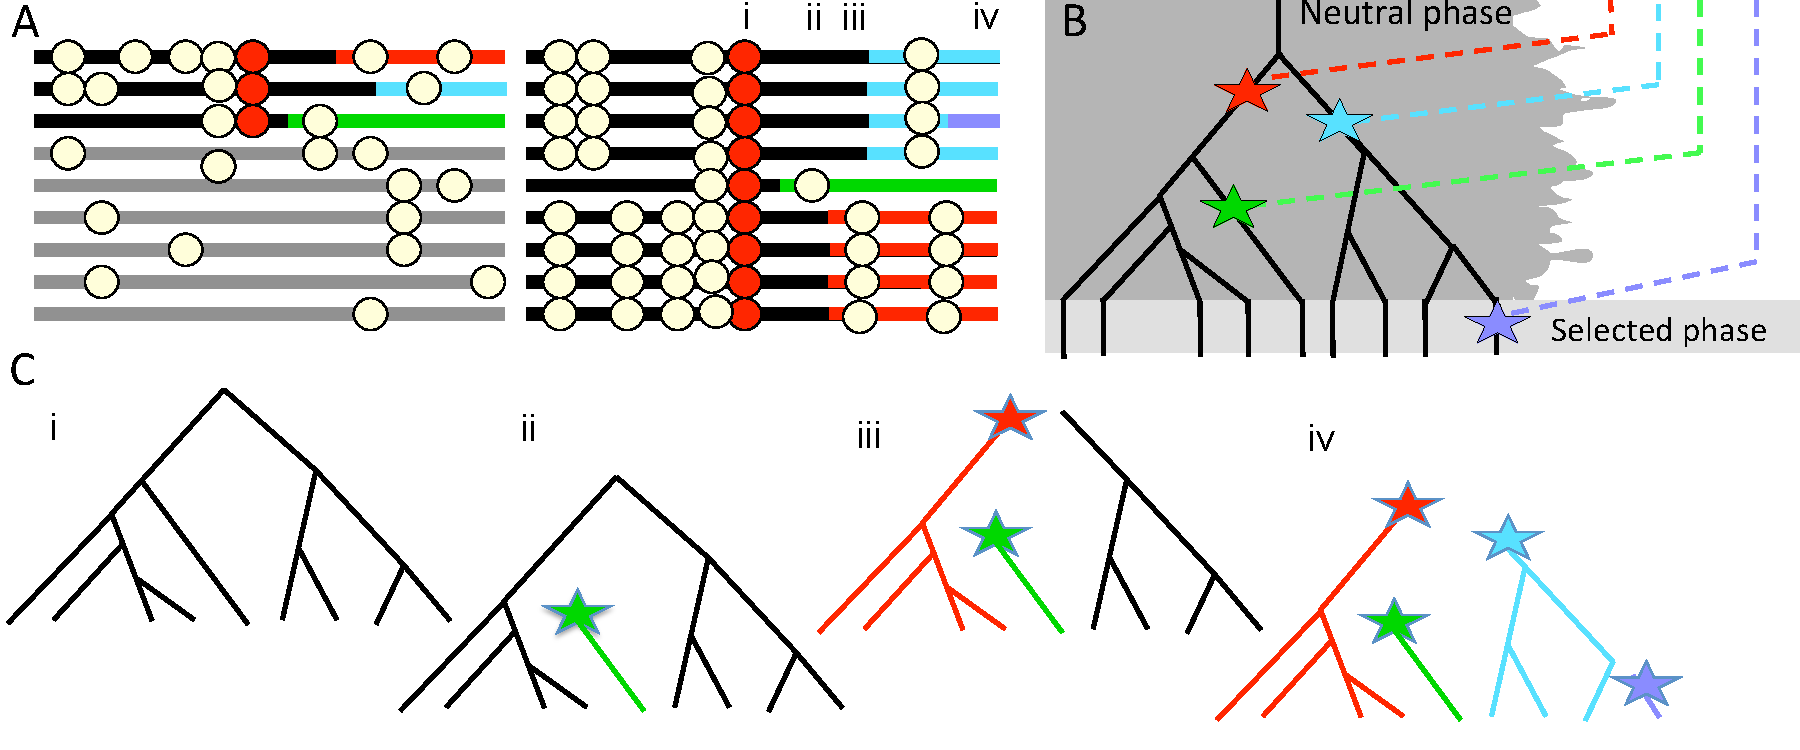
\includegraphics[width = 0.8\textwidth]{../Paper_Figures/Cartoon_of_soft_sweeps.pdf} \label{cartoon_fig_1}
	\caption{caption goes here}
\end{figure}


\subsubsection{Sweep Phase}
Looking backward in time, let $X\left(t\right)$ be the frequency of the B allele at time $t$ in the past, where $t=0$ is the moment of fixation (i.e. $X\left(0\right) = 1; X\left(t\right) < 1\ \forall\ t > 0$). If we consider a neutral locus a recombination distance $r$ away from the beneficial allele, the probability that  fails to recombine off of the selected background in generation $t$ given that it has not done so already is $1-r\left(1-X(t)\right)$. If we let $\tau_{f}$ be the generation in which the environmental change occurred, marking the boundary between the sweep phase and the standing phase (i.e. $X\left(\tau_{f}\right) = f$), then the probability that a single lineage manages to recombine off the selected background at any point during the course of the sweep phase is given by
\begin{equation}
P_{NR} = \prod_{t=0}^{\tau_{f}} 1-r\left(1-X(t)\right)  \approx \exp \left(-r \int_0^{\tau_{f}}(1-X\left(t\right))\mathrm{d} t \right)
\end{equation}
for $r \ll 1$. We set  $\mathcal{T}_{\left(s,f\right)} = \int_0^{\tau_{f}}(1-X\left(t\right))\mathrm{d}t$, so that the probability that a lineage manages to recombine off the selected background during the course of the sweep from frequency $f$ can be written simply as $e^{-r\mathcal{T}_{\left(s,f\right)}}$. If the effect of our beneficial allele on relative fitness is strictly additive, such that heterozygotes enjoy a selective advantage of $s/2$ and heterozygotes an advantage of $s$, then the trajectory of the beneficial allele through the population can be approximated deterministically by the logistic function, such that 
\begin{equation}
	\mathcal{T}_{\left(s,f\right)} = \frac{ln\left(\frac{N_e - 1}{f}-N_e + 1\right)}{s}.
\end{equation}

We assume that the sweep occurs fast enough that the probability of coalescence during the sweep is essentially zero. Therefore, each lineage either recombines off the beneficial background, or fails to do so, independently of all other lineages. The probability that $i$ out of $n$ lineages fail to escape off the sweeping background is the
\begin{equation}
P_{NR}(i \mid n) = {n \choose i} P_{NR}^{i} (1-P_{NR})^{n-i}.
\end{equation}
This binomial approximation has been made by a number of authors in the context of hard sweeps \citep{Barton1998}, and more accurate approximations have been developed \citep{Durrett:2004fl,Durrett:2005fr,Etheridge:2006fk,Messer:2012ie}. However, as long as selection is strong, the sample is not too large,  and $\tau_{f}$ is not too long, then this approximation should be adequate. Other, more accurate approximations could certainly be incorporated into our framework, but we stick with this simple form for the sake of clarity of presentation.

%At a given distance away from the selected site every one of the lineages that recombines out of the selected class will be a singleton, and the remaining lineages will be partitioned according to the Ewens' Sampling formula.  



\subsubsection{Standing Phase}
Looking backward in time, having originally sampled $n$ lineages at $t=0$, we arrive at the beginning of the standing phase at time $\tau_{f}$ with $i$ lineages still linked to the beneficial background, the other $n-i$ having recombined into the non-beneficial background during the sweep.

We will argue that an understanding of patterns of diversity at the neutral locus following a standing sweep can be obtained principally by tracking the histories of only the lineages that are found on the \textbf{B} background at the beginning of the standing phase, and assuming that lineages which recombine off of the \textbf{B} background do not re-enter it. This is obviously a coarse approximation to the true process, but as we argue below, it captures many of the major features sufficiently well for our purposes.

% The following paragraphs are therefore structured as follows: first, we describe an approximation to the coalescent process for \textbf{B} alleles at the \fancyB locus conditional on being at a frequency $f$ at the beginning of the standing phase. Next, we describe an approximation to the process of recombination events which move alleles at the \fancyN locus from the beneficial background onto the non-beneficial background at the \fancyB locus. Finally, we combine these two processes along with the recombination process during the sweep phase and a separation of timescales argument to give an approximate description of the full genealogy at the \fancyN locus.

\paragraph{The Coalescent Process of the B Alleles}

%In attempting to construct the genealogy of the B alleles backward in time, consider that in the first generation of the standing phase, the probability that any pair of B coalesces with one another is $1/\left(2Nf\right)$, while the probability that any pair of b alleles coalesce with one another is $1/\left(2N\left(1-f\right)\right)$. In general, the pairwise coalescent probabilities for pairs of lineages $T$ generations back into the standing phase are $1/\left(2NX(\tau_{f} + T)\right)$ for the B alleles, and $1/\left(2N\left(1-X\left(\tau_{f}+T\right)\right)\right)$ for the b alleles, where the frequency $X\left(\tau_{f} + T\right)$ may be equal to, greater than, or less than $f$, due to the random sampling effects of genetic drift. Further, coalescent events which may have occurred during the intervening $T$ generations contain information about the distribution of $X\left(\tau_{f} + T\right)$.

A number of researchers have studied the behavior of this process \citep{Wiuf1999,Wiuf:2000js} \jb{who else}, either conditional on the frequency of the allele in a sample or in the population. \cite{Wiuf:2000js} has shown that the expected time to the first coalescent event is $2 N f/ {i \choose 2}$ in the absence of other information, e.g. as to whether the allele is ancestral or derived. However, the distribution of coalescence times is no longer exponential. The variance of the time between coalescent events is increased relative to the exponential as a direct result of the fact that the frequency may increase or decrease from $f$ before a given coalescent event is reached. Further, in contrast to the standard coalescent, there is non-zero covariance between subsequent coalescent intervals, as a result of the information they contain about how the frequency of the allele has changed, and thus about the rate at which subsequent coalescent events occur. Lastly, if the allele is known to be either derived or ancestral the coalescent times have a more complicated expectation, as the allele is in expectation either decreasing or increasing in frequency backward in time due to the conditioning on loss or fixation respectively.

%Because we are generally assuming that $f<<1$, the first approximation we make for the standing phase is to assume that no b alleles coalesce until after all of the B alleles have coalesced and the mutation has been removed. 
%
%
%If the beneficial allele were held fixed at this frequency $f$ over a long period into the past, then the genealogy of our $i$ beneficial lineages would simply be a neutral coalescent with pairwise coalescent rate $1/(2 N f)$ (assuming that $f \gg 1/(2N)$ so that the standard coalescent assumptions hold). Such a fixed frequency could result from a beneficial allele that was balanced at low frequency by strong, constant selection. If instead of being held steady at a frequency $f$, the allele is allowed to drift neutrally, this constant coalescent rate no longer holds, and the problem becomes considerably more complicated.


Despite these complications, we have found that assuming that lineages coalesce at a rate $ {i \choose 2}/(2 N f)$ and that coalescent time intervals are independent, i.e. that the allele frequency does not drift from $f$, is not a bad approximation when $f \ll 1$, even when we condition on the allele being derived. In Supp. Figures XXX-XXX we show some comparisons of the coalescent process embedded in a drifting allele frequency and this approximation.

The main reason for using this approximation is that, in conjunction with a separation of timescales (i.e. an assumption that no \textbf{b} alleles coalesce until after all \textbf{B} alleles have), it allows us to work with a simple, well understood caricature of the true process that describes the genealogy at the selected site with reasonable accuracy. Given this simplified coalescent process, we can study the process of recombination events occurring between the adaptive and neutral loci to understand the distribution of the genetic variation at the neutral locus that will hitchhike along with the \textbf{B} allele once the sweep begins. 

\paragraph{Recombination Events Ocurring During the Standing Phase}
We will again rely on the condition that $f \ll 1$, and assume that any lineage at the neutral locus that recombines off of the background of our beneficial allele will not recombine back into that background before it is removed by mutation. Under these assumptions, recombination events which move lineages at the \fancyN locus from the beneficial background onto the non-beneficial background can be viewed simply as events on the genealogy at the \fancyB locus which occur at rate $r\left(1-f\right)$ for each lineage independently. Rescaling time by $2Nf$, an understanding of the genealogy at the \fancyN locus can therefore be found by considering the competing poisson processes of coalescence at rate ${i \choose 2}$, and recombination at total rate $2Nirf(1-f)$

%In Figure \ref{cartoon_fig_1}B we show the coalescent genealogy at the selected site, and show recombination events out of the beneficial allele class imposed on the genealogy (these events are colored to correspond to the events on the haplotypes in Figure \ref{cartoon_fig_1}A). In Figure \ref{cartoon_fig_1}C we show the genealogy at various points along the sequence shown in Figure \ref{cartoon_fig_1}A, between recombination events. 

%Assuming that the frequency of the allele remains fixed at $f$, at a distance $r$ away from the selected site a lineage recombines out of the selected class at rate $r(1-f)$. As coalescent occurs at a rate ${i \choose 2}/(2Nf)$, we can rescale time in units of $2Nf$ so that coalescence happens at a rate ${i \choose 2}$, and recombination events out of the selected class happen at rate $2Nrf(1-f)$.

If we are interested in the number and size of different recombinant clades at a given recombination distance from the selected site (colored clades in Figure \ref{cartoon_fig_1}B \& C) this a direct analogy of the infinite alleles model \citep{}. In the normal infinite alleles process, we imagine simulating from the coalescent, scattering mutations down on the genealogy, and then assigning each lineage to be of a type corresponding to the mutation that sits lowest above it in the genealogy. Alternately, we can create a sample from the infinite alleles model by simulating the mutational and coalescent processes simultaneously: coalescing lineages together as we go move backward in time, ``killing'' lineages whenever they first encounter a mutation and assigning all tips sitting below the mutation to be of the same allelic type (see Figure \ref{cartoon_fig_1}C) \jb{cite for coalescent with killings}.

Given the direct analogy to the infinite alleles model under our set of approximations, the number and frequency of the various recombinant lineage classes at a given distance from the selected site can be found using the Ewens Sampling Formula \citep{Ewens1972}. The population-scaled mutation rate in the infinitely-many alleles model ($\theta/2=2N\mu$), is replaced in our model by the rate of recombination out of the selected class ($R_{f}/2=2Nrf(1-f)$). If $i$ lineages sampled at the moment of fixation fail to recombine off of the beneficial background during the course of the sweep, then the probability that these $i$ lineages coalesce into a set of $k$ recombinant lineages is 
\begin{equation}
	p_{ESF}(k \mid R_f,n)  = S(i,k) \frac{R_f^k}{ \prod_{\ell=1}^{i-1} (R_f +\ell) }  \label{ESF1}
\end{equation}
where $S(i,k)$ is an unsigned Stirling number of the first kind
\begin{equation}
	S(i,k) = \sum_{i_1 + \dots + i_k = i} \frac{i!}{k!i_1\dots i_k}
\end{equation}
These recombinant lineages partition our sample up between themselves, such that each lineage has some number of descendants in our present day sample $\{i_1,i_2,\dots,i_k\}$, where $\sum_{j=1}^k i_j =i$. Conditional on $k$, the probability of a given sample configuration is
\begin{equation}
	p(\{i_1,i_2,\dots,i_k\} \mid k,i) = \frac{i!}{k! i_1\cdots i_k S(i,k)}  \label{ESF2}
\end{equation}
Note that this does not depend on $R_f$, which gives the classic result that the number of alleles is sufficient statistic for $R_f$ (i.e. the partition is not needed to estimate $R_f$).


\begin{figure}
	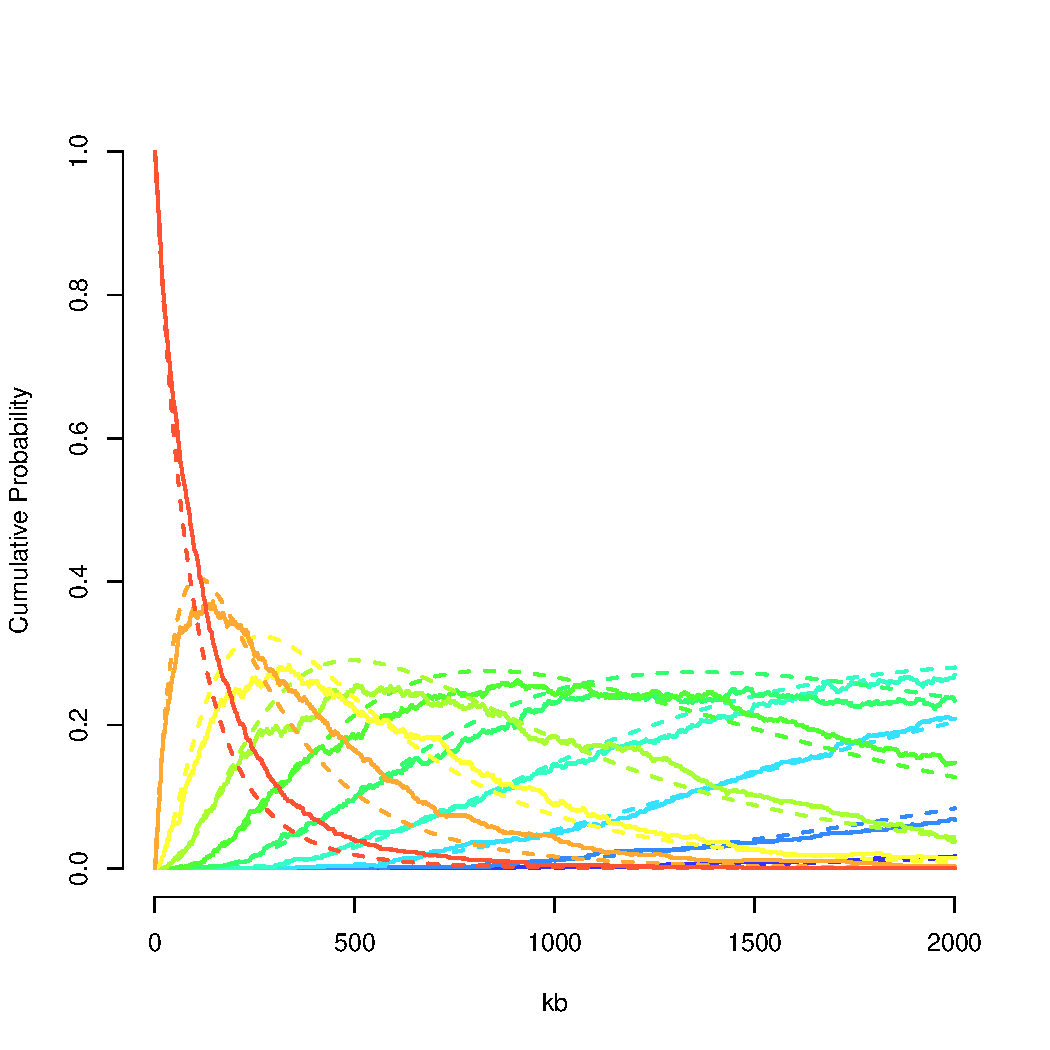
\includegraphics[width = 0.8\textwidth]{../Paper_Figures/Ewens_vs_Jeremy.pdf}
\end{figure}

%and that the number of coalescent families with $1,2,\dots,n$ lineages is given by the partition
%  $\{n_1,n_2,\dots,n_k\}$ is 
% \begin{equation}
% P\left(k,n_1,n_2,\dots,n_n\mid R_f,n \right) =\frac{R_f^i}{ \prod_{j=1}^{i-1} (R_f +j) } \prod_{j=1}^n\frac{1}{j^{n_j}n_j!} \label{ESF}
% \end{equation}
% The probability of there being $k$ alleles (recombinant lineages) in our sample of $n$

\subsubsection*{Patterns of neutral diversity surrounding standing sweeps}
This approximate model of the coalescent for a sweep from standing variation allows us to calculate a number of basic summaries of sequence variation in the region surrounding the sweep. For now we neglect mutations which occur over the time-scale of our shrunken coalescent tree, and assume that all diversity comes from mutations that occurred prior to the sweep, or equivalently that this part of the genealogy contributes negligibly to the total amount of time in the genealogy. This corresponds to an assumption that $2N \mu f \ll 2N\mu$, in line with our previous assumption that $f \ll 1$ (see the appendix for a partial relaxation of this assumption). So long as this assumption holds, we can consider patterns of diversity in our sample at a given site simply by considering properties of the recombinant lineages in our sample, which correspond to alleles drawn independently from a neutral population prior to the start of our sweep.
%
%For example, excluding recombination events during the sweep for a moment, the expected pairwise coalescent time for lineages a distance $r$ away from the sweep is
%\begin{equation}
%	\mathbb{E}(T_2)\approx \frac{1}{1 + R_f} \times 0 + \frac{R_f}{1 + R_f} \times 2N
%\end{equation}
%where the two terms correspond to the contribution from failing to recombine during the standing phase (thereby coalescing very rapidly), and alternately to one or both lineages escaping from the beneficial background and coalescing $2N$ generations ago.
%
%Now incorporating recombination during the sweep, the expected pairwise coalescent time a distance $r$ away from the sweep is
%\begin{equation}
%	\mathbb{E}(T_2) \approx \left(1-\frac{1}{1 + R_f} P_{NR}^2  \right) \times 2N
%\end{equation}
%as to avoid (near) instantaneous coalescence our pair of lineages could either recombine during the sweep or during the standing phase. The expected level of pairwise diversity as we move away from a sweep is given by $2\mu \mathbb{E}(T_2)$ (see Figure \ref{pi_plot} for a comparison of this approximation with coalescent simulations done using $ms$). 
%

%
%\jb{I feel like maybe we should do only diversity and the frequency spectrum in the main body of the paper. Doing pi, S, and SFS feels a bit much.}

\begin{figure}
	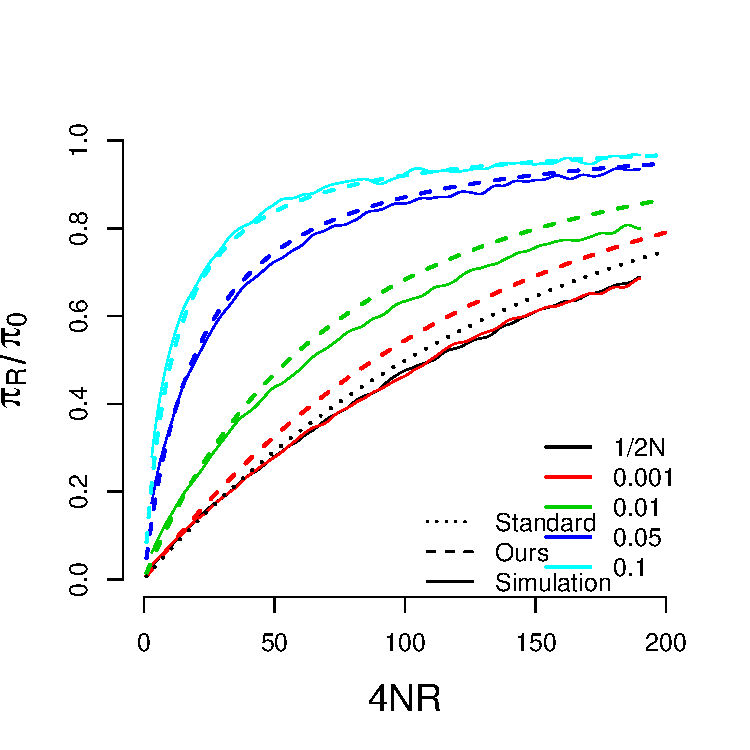
\includegraphics[width = \textwidth]{../Paper_Figures/pi_density.pdf} \label{pi_plot}
\end{figure}

We first take interest in determining the expected total time in the genealogy, at a given distance from the selected site, which allows us to obtain approximations for simple summary statistics such as the pairwise diversity and expected number of segregating sites. Conditional on $m$ independent lineages escaping the sweep, the expected total time in the genealogy is $2N \sum_{j=1}^{m-1} 1/j$, the standard result for a neutral coalescent with $m$ lineages \citep{Watterson:1975ur}. Ignoring for a moment recombination during the sweep phase, the probability that $k$ independent lineages escape during the standing phase is the probability of $k$ alleles in a sample of $n$ under the ESF, $p_{ESF}(k\mid R_f,n)$. If we condition on observing $n-i$ singleton recombinants escape during the sweep phase, then the expected time in the genealogy is
\begin{equation}
	\mathbb{E}(T_{TOT} \mid n-i \textrm{ singleton recombinants})  \approx 2N \sum_{k=2}^i p_{ESF}(k\mid R_f,n)   \sum_{j=1}^{k+n-i-1} 1/j.
\end{equation}
%Reincorporating recombination during the sweep phase, the probability that $k$ distinct lineages have recombined off of the beneficial background between the two phases together is
%\begin{equation}
%	\sum_{i=0}^{k} {n \choose i} P_{NR}^{i} (1-P_{NR})^{n-i} p_{ESF}\left(k-m\mid R_f, i\right),
%\end{equation}
%because if $m$ recombinant lineages are generated during the sweep, then the remaining $k-m$ recombinant lineages have to come from recombination events in the standing phase (we take $p_{ESF}\left(0 \mid R_f,0\right)=1$, and $p_{ESF}\left(0 \mid R_f,i\right)=0\ \forall\ i > 0$). 
Summing over all possible numbers of singleton recombinants during the sweep phase, the expected total time in the genealogy is therefore
\begin{equation}
	\mathbb{E}(T_{TOT})  \approx 2N \sum_{i=0}^{n} {n \choose m} P_{NR}^{i} (1-P_{NR})^{n-i} \sum_{k=1}^i p_{ESF}(k\mid R_f,n)   \sum_{j=1}^{k+n-i-1} 1/j.
\end{equation}
(note that we have taken $p_{ESF}\left(0 \mid R_f,0\right)=1$, and $p_{ESF}\left(0 \mid R_f,i\right)=0\ \forall\ i > 0$; whereas it is typically impossible to obtain a sample with zero alleles, in our case we must define these probabilities to accommodate the case in which all $n$ lineages recombine out during the sweep phase).
and the expected number of segregating sites can be found by multiplying this quantity by the mutation rate. 

For a sample of $n = 2$, we can obtain a simple expression for the expected reduction in pairwise diversity relative to the neutral expectation as
\begin{equation}
	\mathbb{E}\left(\frac{\pi_R}{\pi_0}\right) \approx \left(1-\frac{1}{1 + R_f} P_{NR}^2  \right).
\end{equation}

We can also use our approximation to obtain an expression for the full frequency spectrum at sites surrounding a sweep from standing variation. To break the problem into approachable components, we first consider the frequency spectrum of an allele that is polymorphic within the set of lineages which do not recombine during the sweep (ignoring it's frequency in the sweep phase recominants), and we condition on a fixed number $k$ recombinant families from the standing phase. Borrowing from \cite{Pennings2006} (equation 14 of their paper), if we condition on $j$ out of these $k$ recombinant lineages carrying a derived allele, then we can obtain the probability that $l$ of the $i$ sampled lineages carry the derived allele by summing over all possible partitions of the $i$ lineages into $k$ families such that the $j$ recombinant ancestors carrying the derived mutation have exactly $l$ descendants in the present day
\begin{equation}
p(l \mid j, ~k,~i) = \sum_{\substack{i_1+\cdots +i_j=l \\i_{j+1}+\cdots + i_k=n-l}} p(\{i_1,\dots,i_k\} \mid k, n) = \frac{ {n \choose l} }{ {k \choose j} }\frac{ S(l,j)  S(n-l,k-j)  }{ S(n,k) } \label{ESF_gives_freq_spec}
\end{equation}

Next, we write $q\left(j \mid k\right)$ to denote the probability that $j$ out of the $k$ recombinant families carry the derived mutation. For our purposes, we will assume this distribution follows that of the standard neutral coalescent expectation (i.e. $q(j \mid k) = \frac{1/j}{\sum_{\ell=1}^{k-1}1/\ell}$ gives the probability of $j$ derived alleles in a sample of $k$, conditional on segregation), although an empirical frequency spectrum measured from genome-wide data, as in \cite{Nielsen:2005bla} could also be used. The probability that the derived allele is present in $l$ out of $n$ sampled lineages, conditional on there having been $k$ recombinant families, is then 
\begin{equation}
	p(l \mid k, i ) = \sum_{j=1}^k p(l \mid j,~k, ~i)q(j\mid k).
\end{equation}	
Summing over the distribution of $k$ given by \eqref{ESF1}, we obtain an expression for the frequency spectrum conditional on segregation in the set of $i$ lineages which do not recombine during the sweep as
\begin{equation}
	p(l \mid i) =  \sum_{k=2}^{n}  p_{ESF}(k \mid R_f,i)  \sum_{j=1}^{k-1} q(j\mid k) p(l \mid j,~k, ~i)
\end{equation}
%
%To do this we make use of a trick borrowed from \cite{Kimandstephan}, and subsequently used by \cite{NielsenKimetc}, where the frequency spectrum after a sweep reflects the fact that $k$ recombinant lineages survive through the sweep and these $k$ lineages reflect independent draws from the population frequency. This trick was also used by \cite{Pennings:2006fs} to obtain the frequency spectrum of fully linked variation surrounding a soft sweep from multiple mutations (see the ``Frequency distribution of ancestral variation'' subsection in their ``Analytical Derivations'' section). We will denote the probability of sampling $j$ derived copies of a neutral allele out of a sample of $k$ by $q_{j,k}$, i.e. the neutral frequency spectrum in a sample of $k$. At a neutral site at demographic equilibrium $q_{j,k} = 1/j$ \gc{actually what do we want to do here? Do we want site to be segregating? }, otherwise it could be replaced by the empirical frequency spectrum calculated genome-wide \citep[as in ][]{NielsenKimetc}
%Consider the case where no recombination occurs during the selected phase, in that case the probability of observing a neutral site segregating at a frequency of $l/n$ can be written as
%\begin{equation}
%p(l \mid n) =  \sum_{k=1}^{n}  p_{ESF}(k \mid R_f,n)  \sum_{j=1}^{k} q_{j,k}  p(l \mid k,n) 
%\end{equation}
%where $  p(l \mid k,n) $ is the probability that our $k$ recombinant lineages lead to a sample containing into $l$ derived alleles and $n-l$ alleles when the neutral allele segregates at a frequency of $j/k$ in the population before the sweep. To find this we have to sum over the possible configurations $\{a_1,\dots,a_k\}$ as follows

When we allow for recombination during the sweep, the expression becomes more complex, as we must take into account the fact a mutation may be polymorphic after the sweep even if it is fixed in the set of lineages which hitchhike. Nonetheless, we obtain an expression for the frequency spectrum of 
\begin{equation}
p(l \mid n ) = \sum_{i=0}^n P_{NR}(i\mid  n) \sum_{k=1}^{i} P_{ESF}(k \mid R_f,n-i) \sum_{j=1}^{\text{min}\left(k+n-i-1,\ell\right)} q(j\mid k+n-i) \sum_{g = \text{max} \left( j - k , 0 \right) }^{\text{min} \left( j , \ell , \left(n-i\right) \right)} H(g \mid j,k,n-i) p(\ell-g \mid j-g,k,i) \label{rearrange-anc-freq-spec}
\end{equation}
where
\begin{equation}
	H(g \mid j,k,n-i) = \frac{{n-i \choose g}{k \choose j - g}}{{k + n - i \choose j}}
\end{equation}
gives the probability that $g$ out of $j$ derived alleles are found on singleton recombinants created during the sweep, given that there are $n-i$ singletons, and $k$ recombinant families created during the standing phase. Here $n-i$ lineages recombine out during the selected phase, while the remaining $i$ lineages are partitioned into $k$ families due to recombination and coalescence in the standing phase. Out of the $n-i$ singleton lineages, $g$ of them carry the derived allele, while the remaining $j-g$ copies of the derived allele give rise to $l-g$ derived alleles following the sweep, resulting in a final frequency of  $\frac{l}{n}$ in the present day sample. 

This expression is reasonably accurate except for at sites very near to the selected locus. The reason for this is that our approximation assumes that all variation is ancestral to the beneficial mutation at the selected locus, whereas very close the selected locus, it is unlikely that there have been any recombination events at all, and so any segregating variants which do exist are likely to have arisen as new mutations on the genealogy which sits under the mutation that gave rise to the beneficial allele. Because this genealogy is simply a sample from the standard neutral coalescent with the external branches lengthened by an amount corresponding to the duration of the sweep phase, the frequency spectrum very near to the selected locus is approximately the neutral frequency spectrum with a slight excess of singletons. In the appendix, we give an \textit{ad hoc} expression which takes into account new mutations near the selected locus, and markedly improves our prediction of the frequency spectrum in this region. In figure BLAH, we show a comparison of simulations done in \textit{ms} with the approximation in \eqref{rearrange-anc-freq-spec} and the improved approximation in the appendix.

%\subsubsection{Linkage Disequilibrium}
%\jb{obviously needs more explication of the history of studying LD across sweeps, but will deal with later.}
%\cite{StrobeckMorgan78} and \cite{Hudson85} showed that the expectation of the linkage disequilibrium statistic $D^2$ (i.e. the square of the covariance in allelic state at two loci) can be expressed as
%\begin{equation}
%	D^2 = F_{ij,ij} - 2F_{ij,ik} + F_{ij,kl}
%\end{equation}
%where the three terms are, respectively, the probability that two sequences $i$ and $j$ are identical at both sites $x$ and $y$, the probability that sequences $i$ and $j$ are identical at site $x$ while sequences $i$ and $k$ are identical at site $y$, and finally that sequences $i$ and $j$ are identical at site $x$, while sequence $k$ and $l$ are identical at site $y$. \cite{McVean2002} showed that each of these quantities can be expressed in terms of the expected product of coalescent times with the genealogies at sites $x$ and $y$ for samples with the given configurations
%\begin{equation}
%	D^2 = \frac{Cov\left(t_{x\left(ij\right)},t_{y\left(ij\right)}\right) - 2Cov\left(t_{x\left(ij\right)},t_{y\left(ik\right)}\right) + Cov\left(t_{x\left(ij\right)},t_{y\left(kl\right)}\right)}{\mathbb{E}\left[T_x T_y\right]}
%\end{equation}
%where $t_{x\left(ij\right)}$ is the coalescence time of sequences $i$ and $j$ at site $x$, and $T_x$ is the total height of the genealogy at site $x$. \cite{McVean2002} further obtained an expression for the denominator of $\sigma_d^2$, such that
%\begin{equation}
%	\sigma_d^2 = \frac{Cov\left(t_{x\left(ij\right)},t_{y\left(ij\right)}\right) - 2Cov\left(t_{x\left(ij\right)},t_{y\left(ik\right)}\right) + Cov\left(t_{x\left(ij\right)},t_{y\left(kl\right)}\right)}{\mathbb{E}\left[t_{x\left(ij\right)}\right]\mathbb{E}\left[t_{y\left(kl\right)}\right] + Cov\left(t_{x\left(ij\right)},t_{y\left(kl\right)}\right)}.
%\end{equation}
%Further, because $Cov\left(t_{x\left(ij\right)},t_{y\left(kl\right)}\right) = \mathbb{E}\left[t_{x\left(ij\right)}t_{y\left(kl\right)}\right] - \mathbb{E}\left[t_{x\left(ij\right)}\right]\mathbb{E}\left[t_{y\left(kl\right)}\right]$, and because the expected pairwise coalescent time is the same at each locus for all three sampling configurations, we can cancel all of the terms involving products of expectations to obtain
%\begin{equation}
%	\sigma_d^2 = \frac{\mathbb{E}\left[t_{x\left(ij\right)}t_{y\left(ij\right)}\right] - 2\mathbb{E}\left[t_{x\left(ij\right)}t_{y\left(ik\right)}\right] + \mathbb{E}\left[t_{x\left(ij\right)}t_{y\left(kl\right)}\right]}{\mathbb{E}\left[t_{x\left(ij\right)}t_{y\left(kl\right)}\right]}.
%\end{equation}
%
%We will rely on the assumption that zero time elapses while at least one lineage remains on the background of the selected allele. For clarity, call configurations $\{ij,ij\}$, $\{ij,ik\}$, and $\{ij,kl\}$ states A, B and C respectively, and label as state O any configuration in which ancestral material has been lost due to coalescence at either site. We need to know the expected product of coalescent times for pairs of lineages sampled in each of these three configurations at the moment the beneficial allele fixes. Under our approximation in which coalescence on the selected background (either before or after it actually becomes beneficial) is assumed to happen at $t = 0$, we can calculate the expected product of coalescent times for neutral loci sampled on the selected background at fixation as a function of the probability of transitioning to any other configuration at the first moment when all four alleles are found on the wild type background. For example,
%\begin{equation}
%	\mathbb{E}_S\left[t_{x\left(ij\right)}t_{y\left(ij\right)}\right] = \phi_{AA}\mathbb{E}_W\left[t_{x\left(ij\right)}t_{y\left(ij\right)}\right] + \phi_{AB}\mathbb{E}_W\left[t_{x\left(ij\right)}t_{y\left(ik\right)}\right] + \phi_{AC}\mathbb{E}_W\left[t_{x\left(ij\right)}t_{y\left(kl\right)}\right] + \phi_{AO}\times 0
%\end{equation}
%where $\phi_{AA}$, $\phi_{AB}$, $\phi_{AC}$ and $\phi_{AO}$ are the probabilities of transitioning from state A at $t = 0$ to state A, B, C or O at the first moment when no lineages remain on the selected background, and the expectations with subscript W represent the values obtained for standard neutral theory. These quantities are known 
%\begin{align}
%	\mathbb{E}_W\left[t_{x\left(ij\right)}t_{y\left(ij\right)}\right] = \frac{36 + 14R +R^2}{18 + 13R + R^2} \\
%	\mathbb{E}_W\left[t_{x\left(ij\right)}t_{y\left(ik\right)}\right] = \frac{24 + 13R +R^2}{18 + 13R + R^2} \\
%	\mathbb{E}_W\left[t_{x\left(ij\right)}t_{y\left(kl\right)}\right] = \frac{22 + 13R +R^2}{18 + 13R + R^2}.	
%\end{align}
%Therefore, our only task is to calculate the transition probabilities. \cite{McVean:2006ke} approaches this problem for the standard hard sweep case by separating the sweep into two components. In the first part of the sweep (looking backward in time), each lineage makes an independent choice whether to recombine out of the sweep or not, recombining out with probability $(1 - e^{-\frac{r}{s}ln(2N)})$. In the second phase of the sweep, all lineages which fail to recombine out are forced to coalesce with probability one, and then mutate out of the selected background immediately.
%
%In order to obtain an expected value for $\sigma_d^2$ following a sweep that begins from frequency $f$, we need to modify \citeapos{McVean:2006ke} approach. The first modification is to replace the probability of recombining off of the selected background with $(1 - e^{-\frac{r}{s}ln(\frac{1}{f})})$ reflecting the fact that the selected phase is slightly shorter when mutations come a frequency greater than $\frac{1}{2N}$, and thus there is less opportunity to recombine. The second modification is more involved. In contrast to \citeapos{McVean:2006ke} hard sweep model in which no recombination occurs during the second phase, in our model we must track the behavior of a Markov chain in which coalescence, recombination, and mutation may occur. The set of events which we allow to occur in this Markov chain are recombination of an allele at the $x$ locus off of the selected background (at rate $r_x\left(1-f\right)$), recombination at the $y$ locus off of the selected background (at rate $r_y\left(1-f\right)$), coalescence of two chromosomes on the selected background (at rate $\frac{1}{2Nf}$), and coalescence of two chromosomes on the non-selected background (at rate $\frac{1}{2N\left(1-f\right)}$), and mutation off of the selected background, which we assume to occur with probability one as soon as there is only a single chromosome left on the selected background.
%
%This Markov chain has a total of 46 states which can be reached beginning from one of the three initial configurations (A, B or C). However, 26 of these transitions result in loss of ancestral material due to coalescence, and thus contribute a value of zero toward the product of coalescence times. We therefore don't need to explicitly calculate the probability of transitioning into these states, and need only track transitions to states that don't result in loss of ancestral material. The full transition matrix \jb{will be} given in the Appendix, but here are a few of the transition probabilities as examples
%\begin{align}
%	&P\left(\{i^Sj^S,k^Sl^S\} \rightarrow \{i^Sj^S,k^Sl^W\}\right) = \frac{4Nr_y f\left(1-f\right)}{12 + 4Nr_x f\left(1-f\right) + 4Nr_y f\left(1-f\right)} \\
%	&P\left(\{i^Sj^W,k^Sl^W\} \rightarrow \{i^Sj^W,i^Sk^W\}\right) = \frac{1}{1 + \frac{f}{1-f} + 2Nr_x f\left(1-f\right) + 2Nr_x f\left(1-f\right)} \\
%	&P\left(\{i^Sj^S,i^Sk^S\} \rightarrow \{i^Sj^W,k^Sl^S\}\right) = \frac{2Nr_x f\left(1-f\right)}{6 + 2Nr_x f\left(1-f\right) + 2Nr_y f\left(1-f\right)} \\
%	&P\left(\{i^Sj^S,i^Sk^S\} \rightarrow \{i^Sj^W,k^Wl^S\}\right) = 0 \\
%	&P\left(\{i^Sj^W,i^Sk^W\} \rightarrow \{i^Wj^W,i^Wk^W\}\right) = 1.
%\end{align}
%Let $\mathbf{D}$ be the $20\times 20$ transition matrix for the standing phase, and let $\mathbf{A}$ be the transition matrix for the selected phase. 


\subsection{Patterns of Haplotypic Variation}

%\jb{Write some nice intro here}
%Consider the task of both detecting and distinguishing selective sweeps of the classical ``hard'', standing, and multiple hit ``soft'' cases. A large number of methods now exist for detecting classic hard sweeps \jb{refs}, and a few approaches designed specifically for soft sweeps have been developed as well \jb{cite Nandita and Ben here}.
%
%We consider the problem of doing inference on sweep parameters (where the ``type'' of sweep is included as a ``parameter'') in a hypothetical situation in which we have access to the maximal amount of information which could reasonably be obtained directly from sequence data. In other words, we imagine an ``infinite haplotypes'' model, in which all chromosomes sampled at the completion of the sweep can be assigned to a unique ancestral chromosome which existed immediately prior to the beginning of the sweep. 

We have described a model for the marginal genealogical and recombinational history at a site some distance from a standing sweep. It is of interest to consider patterns of haplotypic diversity we expect to observe along the sequence for a single realization of a standing sweep, or in other words the \textit{joint} history of the sequence in the region surrounding beneficial allele. If we again follow the custom of first ignoring recombination during the sweep phase  We want to be able to describe patterns of haplotypic variation surrounding standing sweeps. In particular, we are interested in the usefulness of haplotype statistics to distinguish three different types of ``full sweep'': the classical hard sweep, a sweep including multiple mutations, and a sweep from standing variation. 

%We adopt the convention of querying the number and partition of haplotypes which are present within a window with the left boundary at the position of the selected mutation, and the right boundary some distance away. We will argue that the majority (but not all) of the information which can be used to distinguish these types of sweeps can be accessed by considering how the number and partition of haplotypes changes as the right boundary of the window is increased from zero until we reach the point at which all chromosomes are present on distinct haplotypes (the point beyond which there is no further information about the sweep).

We continue our infinitely-many haplotypes perspective, in which we imagine that every piece of DNA present in the sample taken at fixation can be labelled/colored according to which chromosome in the ancestral, pre-sweep population it traces its ancestry to. Under this convention, right at the selected site, all chromosomes descending from either a hard sweep or a standing sweep will be of the same ``color'', due to their shared common ancestry, while for multiple mutation soft sweeps each set of chromosomes tracing to a different mutational origin of the beneficial allele will be of a different color. For all kinds of sweeps, the number of distinctly colored haplotypes increases with distance from the selected site due to recombination events which cause transitions along the sequence in the haplotype partition scheme.

With this perspective, most of the information about the parameters of the sweep (including that of which type of sweep it is), are contained jointly in the set of transitions in the haplotype partition scheme as one moves away from the selected site, along with the list of their locations along the sequence. As we are considering the haplotype partition largely in the context of inference, it is worth briefly acknowledging that by envisioning detailed knowledge of haplotype identities and transitions around a selected site, we are assuming access to a level of data that is quite unlikely to be attainable in any real population. The following results therefore constitute a sketch of the upper bound on the ability to distinguish the different kinds of sweeps. In cases where the ancestral genetic diversity is low, the problem is considerably worse.

Below, we consider the construction of this haplotype partition as a process along the sequence for each of the three types of sweeps, beginning with either a single haplotype at the selected site (hard and standing cases), or potentially more than one (in the multiple mutation case), and transitioning as we move away through states where there are two, three, four, etc. haplotypes, until we eventually transition through to the state where all sampled chromosomes are found on independent haplotypes. 

%For both hard sweeps and standing sweeps, all chromosomes at the selected site trace their ancestry to the individual ancestral chromosome on which the beneficial mutation originally arose, and thus there is only a single haplotype at the selected site. As we imagine moving along the sequence away from the selected site, we would encounter a transition from a single haplotype to two haplotypes (with some number of chromosomes partitioned into each haplotype group), and a subsequent transition from two haplotypes to three haplotypes (which arises from splitting one of the two existing haplotypes into two subgroups). If we consider moving further and further out from the selected site, we would eventually reach the point where there were $n$ distinct haplotypes in a sample of $n$ chromosomes, where each subsequent increase in the number of haplotypes as we move away from the selected site results from a partitioning of one existing haplotype into two sub-haplotypes.

%In principle, then, all of the information about a given sweep is contained in the distances at which transitions in the partition scheme occur, as well as the path the sequence takes through partition space (e.g. whether the first transition creates a partition of \{6,4\} or \{7,3\}, etc.)

%These transitions arise due to recombination events in on the (unknown) genealogy as we move away from the selected site. Continuing to ignore neutral mutations which have occurred since the mutation(s) which gave rise to the sweep, all of the information about the sweep is contained jointly in the distances 

%\jb{Note that there is also additional information present in the locations and frequencies, and correlations between mutations which have occurred on the background of the beneficial allele. We will focus for the most part on the haplotype partition scheme as defined solely by recombination events, and then comment briefly on the role of new mutations occurring on the beneficial background.}

\begin{figure}
	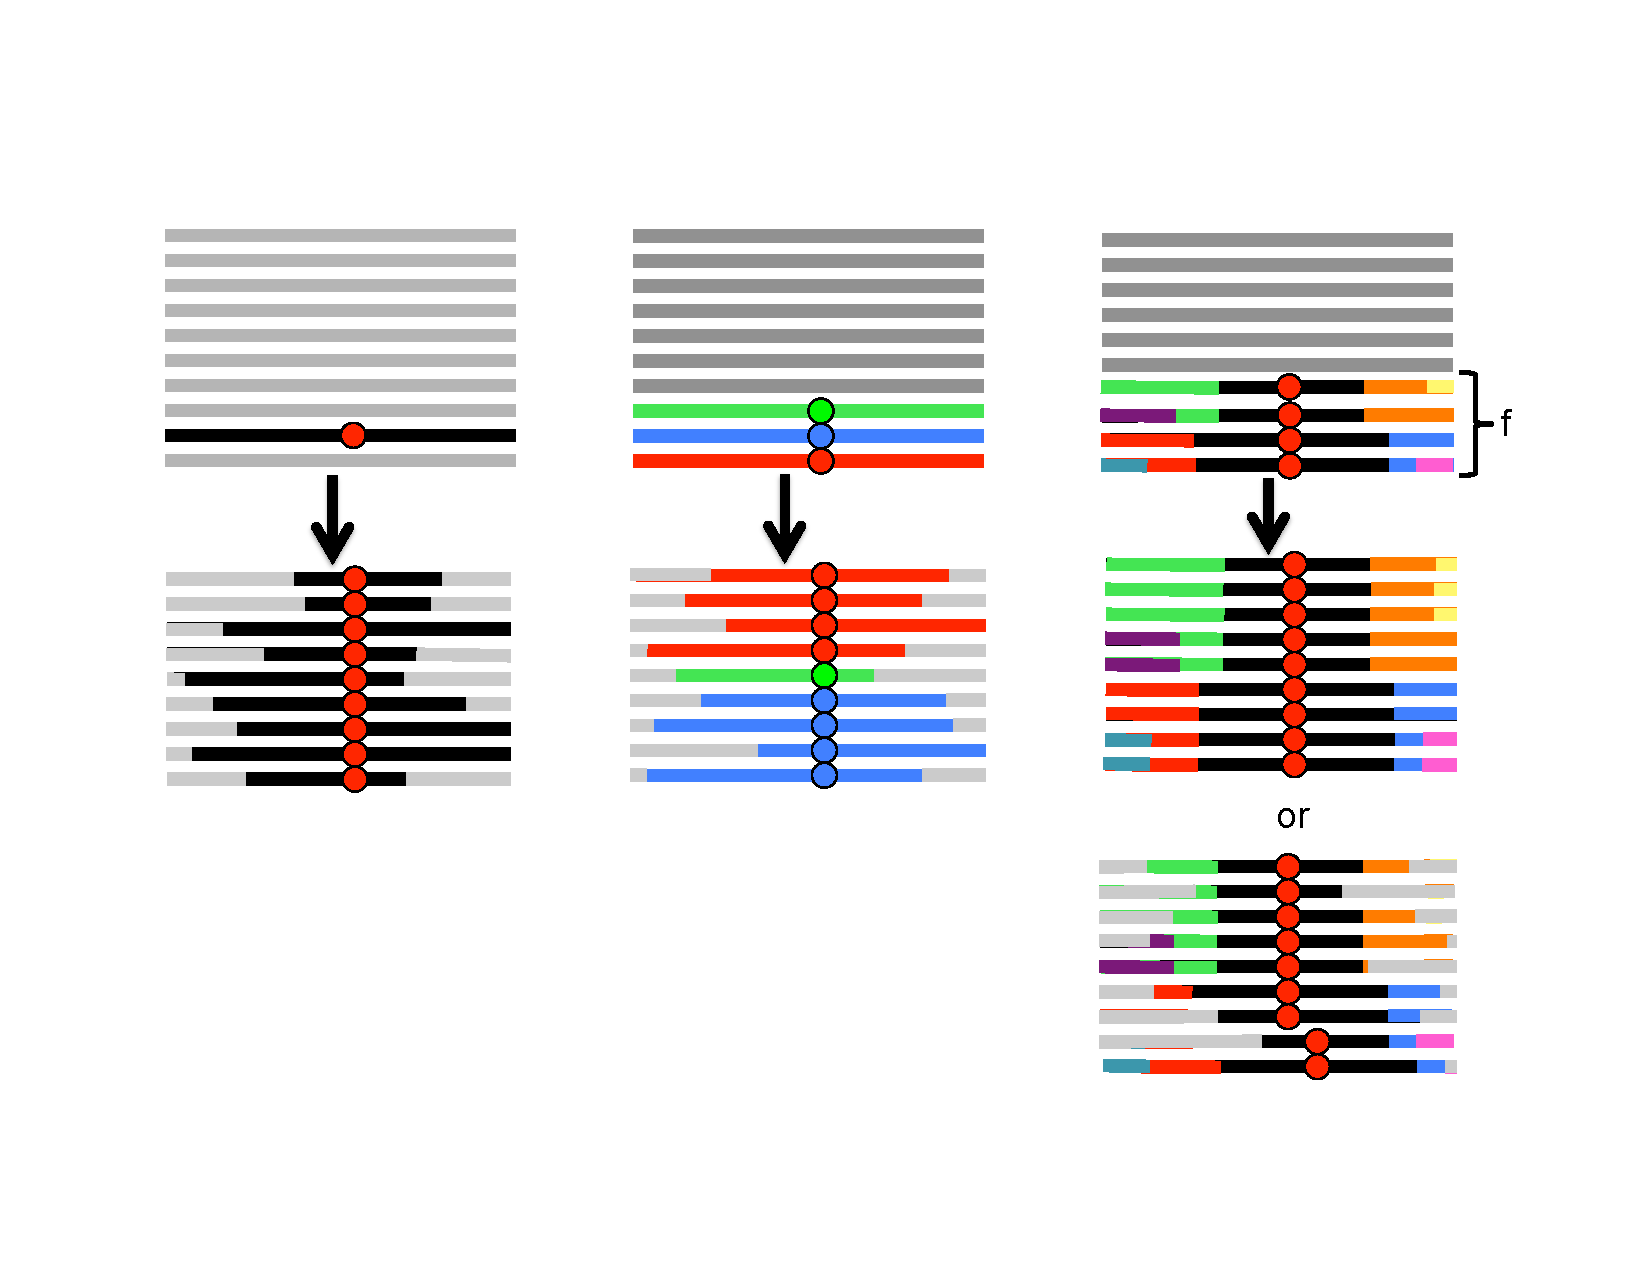
\includegraphics[width = 0.8\textwidth]{../Paper_Figures/three_kinds_of_sweep.pdf} \label{cartoon_3_kinds}
	\caption{caption goes here}
\end{figure}


\paragraph{The Classic Hard Sweep Case}

Under the binomial approximation for the classic hard sweep case, as used by \cite{Fay:2000usa,others}, the expected distance in base pairs to the transition from one haplotype to two is $\frac{1}{n\mathcal{T}_s r_{BP}}$, and in general the expected distance between the transition from $i$ haplotypes to $i+1$ haplotypes is $\frac{1}{\left(n-i+1\right)\mathcal{T}_s r_{BP}}$. Further, conditional on the value of $\mathcal{T}_s$, the distances between subsequent haplotype partitions are roughly independent. In this approximation, all transitions result from one individual from the core haplotype becoming a singleton due to a recombination event that occurred before the multiple merger at the beginning of the sweep, and thus all of the information about the sweep is contained in the joint distribution on the distances at which the transitions occur. Each of the transitions from grey to black in Figure \ref{cartoon_3_kinds} represents an independent recombination event, and each grey haplotype is randomly drawn from the diversity prior to the sweep.

The majority of our information for identifying full sweeps therefore comes from the presence, and slow decay, of a single haplotype over long distances. The fact that recombination is slowly peeling off singleton haplotypes as we move away from the sweep results in the signal of an excess of singletons and high frequency derived alleles \citep{Fay:2000usa} occurring in genomic run, a signal which forms the basis for a number of popular sweep detection algorithms \cite{Sweepfinder,EHH,etc}. Another consequence of this behavior is that immediately following a full sweep, there is a much reduced level of pairwise linkage disequilibrium across the selected site \citep{Stephan2006,McVean:2006ke}, as the star-like tree at the selected site renders recombinations on either side of the sweep effectively independent \citep{McVean:2006ke}.

In reality, all coalescence does not occur instantaneously at the base of a classic hard sweep, especially when the sample is even moderately large (i.e. $n > 20$), and thus there is an opportunity for recombination events to occur on internal branches of the genealogy \cite{Etheridge06,Barton98}. This causes transitions in the partition scheme that result in a class of additional non-singleton haplotypes, which eventually break apart farther out from the selected site due to additional recombination events lower down in the genealogy.

\paragraph{Sweep with multiple mutations.}
\citet{Pennings2006a, Pennings2006} investigated the case of multiple mutations at a single selected locus contributing to a sweep. This sort of sweep can occur if there are multiple mutations present at mutation-selection balance prior to the onset of selection, or if they arise sequentially during the sweep. The simple signal of hitchhiking in this case is complicated, as rather than a single allele sweeping to fixation, the multiple alleles all sweep to somewhat intermediate frequencies, partitioning the same into multiple core haplotypes. For example, in Figure \ref{cartoon_3_kinds}B, the sampled haplotypes have been partitioned by multiple mutations during the sweep into three distinct haplotypes at the selected site. Parameterizing the mutation rate toward beneficial alleles at the locus as $\mu_{B}$, \cite {Pennings2006a} found that for small samples and strong selection, the partitioning of lineages at the selected site by different mutations was well approximated by the Ewens Sampling formula with parameter $4N_e\mu_B$. Clearly, if a particular stochastic realization of this process results in only a single mutation, then we simply have a classic hard sweep, as above.

The tree under each of these mutations will be a very short and reasonably star-like, such that there will be a single haplotype associated with each mutation close to the selected site. Aside from the presence of multiple haplotypes in this core region, the breakdown in the haplotype partition moving away from the selected locus is relatively similar to that under the hard sweep. Again assuming the sweep took $\mathcal{T}_s$ generations, the distance between the $i^{th}$ and $i+1^{st}$ haplotype transitions is exponential with expectation $\frac{1}{\left(n-i+1\right)\mathcal{T}_s r_{BP}}$.

Allelic differences between ancestral haplotypes at neutral sites will now be found at intermediate frequency in the sample, such that the frequency spectrum can be skewed close to the center of the sweep \citep{Pennings2006}. 
%Thus instances of partial sweeps can be associated with an excess of intermediate frequency alleles close to the sweep \gc{true?}. 
We also anticipate the generation of considerable linkage disequilibrium both between sites on the same side, as well as opposite sides of the sweep due to the correlation induced by the partitioning at the core region\cite{Pokalyuk:2011kq}.  Whether these patterns are visible depends on the magnitude of neutral diversity in the population before the sweep. If the distance between neutral polymorphisms is $\ll 1/(\mathcal{T}_s r_{BP})$ then there will likely be multiple neutral alleles revealing the haplotype partitioning at the selected site, while if this condition is not met, we are unlikely to see the signal of the sweep at all.

\paragraph{Standing Sweep Case}

The situation for a standing sweep is considerably more complicated than either the hard sweep or the multiple mutation sweep. Recall that $\tau_{f}$ gives the duration of the sweep phase, while the time from the beginning of the standing phase back to the common ancestor of the beneficial alleles is approximately $4N_e f$. Therefore, if $4N_e f \ll \tau_{f}$ (i.e. selection is very weak, or the mutation is still quite rare when selection switches on), most of the recombination events that affect the haplotype partition occur during the sweep phase, and so the pattern is very similar to that of a hard sweep.

%If $4N_e f$ is at least on the same order as $\tau_{f}$, then recombinations during the standing phase may contribute to haplotypic patterns surrounding the sweep, whereas if . Figure \ref{cartoon_3_kinds}C shows both a case where $4N_e f \gg \tau_{f}$ and where they are on the same order. We will first consider the case where $4N_e f \gg \tau_{f}$, in which case all of the recombination events affecting the haplotype partition occur during the 

The alternate extreme, where $4N_e f \gg \tau_{f}$, occurs when selection is strong or the mutation was segregating at a relatively high frequency prior to the onset of selection. In this parameter regime, the sweep phase occurs fast enough that recombination events from this period tend to be far away from the selected site, and the structure of the haplotype partition is dominated by the standing phase.

While an analytical treatment of this process is beyond our reach, we can still imagine constructing the haplotype partition as a process along the sequence, which yields some insight. If the total time in the coalescent tree in the neutral phase at the selected site is $T_{tot}$, then the distance to the first recombination is $\sim \exp \left( r_{BP} T_{TOT} \right)$. Using the standard approximation to the constant in Watterson's $\theta$, the expected length scale over which a single haplotype should persist away from the selected site is $\approx 1/( 2 N_e R_f log(n-1))$. This recombination partions the haplotypes according to the infinite alleles model for single mutation placed at random on the geneaology at the selected site (e.g. the green recombinant moving to the left in Figure \ref{cartoon_3_kinds}C). Moving on down the sequence we then generate the next distance to a recombination along the sequence, again from $\sim \exp \left( (r_{BP} T_{TOT} \right)$. We once again uniformly simulate a position on the tree for this new recombination, however, this time only a recombination on some of the branches would result in another colored haplotype being introduced into the sample, e.g. a recombination that falls on the same branch as the previous one. If the recombination falls in a place that doesn't alter the configuration we ignore it, otherwise we split our sample configuration again. For example, the red recombinant in Figure \ref{cartoon_3_kinds}C does not alter the sample configuration and so can be ignored. While it does recombine the selected allele off of its original black haplotype, this recombinant is not visible in our contemporary sample (likewise the light blue recombinant in Figure 1XX is not visible). We iterate this procedure moving away from the selected site, generating exponential distances to the next recombination, placing the recombination down, updating the configuration if needed, until we reach the point that every colored haplotype is a singleton. We then repeat this procedure on the other side of the selected site using the same underlying tree at the selected site. 

An equivalent way to describe this process is to simulate distances to the next recombination that alters the configuration, given the tree. To do this we consider the total time in the tree where a recombination would alter the configuration. Numbering these recombinations out from the selected site,  we start at the selected site $i=0$, with $T_0 = T_{TOT}$ and generate a distance to the next recombination $\sim \exp(r_{BP} T_0)$. We place the recombination on the tree, then prune the tree of branches where no further change in sample configuration could result in a new colored haplotype. We then set $T_i$ to the total time in this pruned tree and carry on this process till we have pruned the entire tree (at which point the distance to the next visible recombination would be infinite as we are left only with singleton haplotypes). 

As we have discussed above, marginally at a given site the partitioning of haplotypes (integrating out the unobserved genealogy) is given by the ESF. It is unclear to us how to couple together the partitioning at two sites in an analytically tractable way, i.e. how to calculate the probability of  how the sample configuration $ \{i_1,i_2,\dots,i_k\},$ is further subdivided by recombinations at a site further along the sequence. Obviously this can be calculated by resorting to brute force integration over the set of all unobserved trees that are consistent with the partition at the first site, but it seems like a more elegant solution could be available. Given the general interest in the ESF motivated by exchangeable partitions and clustering algorithms, such a coupling may be of wider interest.
 
Under our approximation, each of our coloured haplotypes represents an independent draw from the haplotypes present before the sweep, such that allelic differences we see between these ancestral haplotypes are the alleles that segregate after the sweep. As such, we should expect LD to be created between variants on the same haplotypic background. As haplotype configurations should extend over distances $\sim 1/(r_{BP} N_e f)$ this LD will extend over distances unusual compared to background LD if $N_e f \ll N_e$. The colored haplotypic patitioning on either side of the selected site is correlated due to the underlying dependence on the genealogy at the selected site, thus there can be LD across the selected site--unlike the full sweep model. But in contrast to the soft sweeps model we have to wait until we get a sufficient distance from the selected site in order for recombination to have occurred, to have variation to observe the LD. We have explored approximating the pairwise LD around the sweep using the coalescent approach of \citet{McVean:2006ke}, however, we found that no simple expressions were forthcoming from that approach (principally because we have not been able to couple two sites together other than by brute force).

If $\tau_{f}$ is on the same order as $4N_e f$ then the distances to recombination events in the two phases will be on the same genomic scale, but recombinations in the selected phase occur first moving backward in time and so obscure the patterns of the sample described above (see grey bars in Figure \ref{cartoon_3_kinds}Cii). As before the physical distance along the sequence to each recombination during the selected phase is independently $\sim \exp(r_{BP} \tau_{f}) $, such that the core region swept clean of diversity to be  $\sim \exp \left( R_f T_{tot} + r_{bp} n t_{f} \right)$. The ability to see the colored haplotype structure will depend strongly on the exact magnitude of $\tau_{f}$ as compared to $N_e f$, and is likely to be highly stochastic across replicates.


\subsection{Inference Concerns}

Some authors have developed methods to infer the existence of standing sweeps \citep{Peter:2012hta} or multiple hit soft sweeps \citep{Garud:2013ve}. Here, we apply our model of a standing sweep to understand the limitations to inference of standing sweeps and to explore issues of potential confounding between standing and multiple hit soft sweeps.

If $f N_e$ is not a lot smaller than $N_e$ then the resulting sweep will be very hard to distinguish from neutral patterns of diversity, much like the difficulty of identifying weak full sweeps. Obviously we can still potentially identify the allele as a putative signal of selection, if we also identify it as an unusually large change in allele frequencies between populations. In that case the lack of a haplotype signal may alter us that the allele potentially swept from standing variation. In the absence of data from populations where the allele has not swept, we are restricted to identifying alleles where $f N_e + \tau_{f} \ll N_e$. In that case the core region swept clean of variation should usually be distinguishable from background fluctations in diversity (controling for mutation rate, e.g. via divergence data). However, the trough in diversity will be smaller than an equivalent classic sweep with $t_S \approx \tau_{f}$ if $f \gg 1/(2N_e)$. A sweep consisting of multiple adaptive alleles will not result in a region swept clear of diversity, as there is no one core haplotype.

Approaches that are based on looking for an unusually long persistance of haplotypes REFS should have much better power to identify all three kinds of sweep. If $\theta_B$ is not too large, or equivalently if $N_ef$ is on the order of $t_f$ or smaller, then we should have multiple pairs (or higher) of haplotypes that match each other out to a genetic distance of $\sim 1/s$. Obviously the cluster of similar haplotypes is larger in the case of a classic sweep, and so it will likely be hard to design a test that has roughly uniform power over all three types of sweep (particularly the type of sweep from standing variation).

One key signal of a full sweep has been the prescence of singleton (or low frequency) recombinants off the sweep, leading to high frequency derived variants and contributing to the excess of singleton alleles. If the majority of our singleton recombinants arose


\subsubsection{Are $s$ and $f$ independently inferable?}

In our standing sweep model, the information indicating that the sweep began from standing variation comes primarily from an observation that the genealogy at the selected site is shrunken by a factor $f$, while the information about the sweep comes form of the external branches of this genealogy being slightly longer than expected under this rescaling. The task of an inference procedure designed to identify standing sweeps is then to determine both that this shrunken genealogy exists (and that it is smaller than would be expected under neutrality), and that its external branches are too long, given the times in the rest of the tree.

Under our simplified model, 

\gc{points to hit}

Are s and f distinguishable or both inferable.
--Weak selection maybe everyone recoms out
--Large f maybe no signal of sweep?
--What fraction of the singleton recombinants come from selected vs stand phases?
--Do you get to see the singleton recombinants from the sweep. Total coalescent time in sweep phase vs total time in standing phase?

Comparison to multiple mutations. 
--What makes the two cases distinguishable
--Code up? Pennings and Hermisson.


Time since to sweep. 
--does this mess things up?
--scale of recombination and coalescence leading up to sweep.
--Maybe just have this discussion.


\section{Discussion}

Gene conversion --minor point in discussion too. 


%%%%%%%%%%%%%%%%%%%%%%%%%%%%
\section{Acknowledgements}

\section{Methods}


\bibliographystyle{genetics}
\bibliography{library,morelibrary}

\section{Supplementary materials}

\setcounter{table}{0}
\renewcommand{\thetable}{S\arabic{table}}
\setcounter{figure}{0}
\renewcommand{\thefigure}{S\arabic{figure}}

\end{document}
